\documentclass[a4paper]{article}

\usepackage[margin=2.5cm]{geometry}
\usepackage[pdftex]{graphicx}
\usepackage[utf8]{inputenc}
\usepackage[T1]{fontenc}
\usepackage{textcomp}
\usepackage{babel}
\usepackage{amsmath, amssymb}
\usepackage[colorlinks=true,linkcolor=blue]{hyperref}
\usepackage{float}
\usepackage{mathrsfs}
%\usepackage{enumitem}
\usepackage{bbm}
\usepackage{todonotes}

\newcommand{\incfig}[2][1]{%
\def\svgwidth{#1\columnwidth}
\import{./figures/}{#2.pdf_tex}
}


% figure support
\usepackage{import}
\usepackage{xifthen}
\pdfminorversion=7
\usepackage{pdfpages}
\usepackage{transparent}

\pdfsuppresswarningpagegroup=1

\setlength\parindent{0pt}

\newcommand{\qed}{\tag*{$\blacksquare$}}
\newcommand{\qedwhite}{\hfill \ensuremath{\Box}}

%Inequalities
\newcommand{\cycsum}{\sum_{\mathrm{cyc}}}
\newcommand{\symsum}{\sum_{\mathrm{sym}}}
\newcommand{\cycprod}{\prod_{\mathrm{cyc}}}
\newcommand{\symprod}{\prod_{\mathrm{sym}}}

%Linear Algebra

%Redeclaring Span and image
\DeclareMathOperator{\Span}{span}
\DeclareMathOperator{\Ima}{Im}
\DeclareMathOperator{\diag}{diag}
\DeclareMathOperator{\Ker}{Ker}

%Row operations
\newcommand{\elem}[1]{% elementary operations
\xrightarrow{\substack{#1}}%
}

\newcommand{\lelem}[1]{% elementary operations (left alignment)
\xrightarrow{\begin{subarray}{l}#1\end{subarray}}%
}

%SS
\DeclareMathOperator{\supp}{supp}
\DeclareMathOperator{\Var}{Var}

%NT
\DeclareMathOperator{\ord}{ord}

%Alg
\DeclareMathOperator{\Rad}{Rad}
\DeclareMathOperator{\Jac}{Jac}

\DeclareMathAlphabet{\pazocal}{OMS}{zplm}{m}{n}
\newcommand{\unif}{\pazocal{U}}

\begin{document}
    

\subsection*{Class 2}

\textbf{Goal of topology:} define invariants of top. spaces. Find out when
2 spaces are equivalent. Very rarely a complete classification.\\
\linebreak
\begin{center}
    Need a source of spaces to consider. Need methods to tell if two spaces are
    equivalent.
\end{center}

\textbf{Note:} Metric graphs and outer space.


\section*{Chapter 1}
\subsection*{Paths and homotopy}
Setup: A path in a space $X$ is a continuous map $f  \colon I \to X$.\\
A path $f  \colon I \to X$ such that $f(0) = f(1) = x_0 \in X$ is called
a loop, and the common starting and ending point $x_0$ is referred to as the
basepoint. The set of all homotopy classes $\left[ f \right] $ of loops
$f  \colon I \to X$ at the basepoint $x_0$ is denoted $\pi_1 (X, x_0)$.\\
\linebreak
\textbf{Proposition 1.3:} $\pi_1(X,x_0)$ is a group with respect to the product
$\left[ f \right] \left[ g \right]  = \left[ f\cdot g \right] $ where
\[
f \cdot g (s) = \begin{cases}
    f(2s), & 0 \le s \le \frac{1}{2}\\
    g(2s - 1), & \frac{1}{2} \le s \le 1.
\end{cases}
\]
Let a reparametrization of a path $f$ be a composition 
$f \varphi$ where $\varphi  \colon I \to I$ is any continuous map such that
$\varphi(0) = 0$ and $\varphi(1) = 1$.\\
\linebreak
Then given paths $f,g,h$ with $f(1) = g(0), g(1) = h(0)$, we want
a reparametrization $\varphi  \colon I\to I$ such that
$f \cdot (g\cdot h)$ is a reparametrization of 
$\left( f \cdot g \right) \cdot h$; i.e. we want
$f \left(4 \varphi(\frac{1}{2} \right) = f(1)
$, so $\varphi (\frac{1}{2}) = \frac{1}{4}$.
Then
$g\left( 4 \varphi(\frac{3}{4}) - 1 \right) = g(1)$ so
$\varphi \left( \frac{3}{4} \right) = \frac{1}{4}$ and
$h\left( 2 \varphi(1) - 1 \right) = h(1)$ so $\varphi(1) = 1$.
Then
\[
\varphi (t) = \begin{cases}
    \frac{1}{2}t, & t\in \left[ 0, \frac{1}{2} \right] \\
    t - \frac{1}{4}, & t \in \left[ \frac{1}{2}, \frac{3}{4} \right] \\
    2t - 1, & t \in \left[ \frac{3}{4}, 1 \right] 
\end{cases}
\] 

gives $f \cdot \left( g\cdot h \right) \varphi
= \left( f\cdot g \right) \cdot h$.
Hence $(f\cdot g) \cdot h \simeq f\cdot \left( g\cdot h \right) $.
Thus the product in $\pi_1 (X,x_0)$ is associative.\\
To make $\pi_1 (X,x_0)$ into a group, we msut also show identity and inverse:\\
given $f  \colon I \to X$ a path, let $c$ be the constant path at
$f(1)$, so $c(s) = f(1)$ for $s \in I$. Then
$f \cdot c = f \varphi$ with $\varphi 
= \begin{cases}
    2t, & t \in \left[ 0,\frac{1}{2} \right] \\
    1, & t \in \left[ \frac{1}{2},1 \right].
\end{cases}$.
Similarly, for $c (s) = f(0)$, we have
$c \cdot f = f \varphi$ with
$\varphi (t) = \begin{cases}
    0, & t \in \left[ 0, \frac{1}{2} \right] \\
    2t - 1, & t \in \left[ \frac{1}{2},1 \right] 
\end{cases}$.
Thus $c \cdot f \simeq f \simeq f \cdot c$, so the homotopy class
of the constant path at $ x_0$ is a two-sided identity
for $\pi_1 \left( X, x_0 \right) $.\\
\linebreak
Now, letting $\overline{f}(s) = f(1-s)$, we have
$f \cdot \overline{f} $ is homotopic to the constant path by the homotopy
$f_t \cdot g_t$ with $f_{t}(s) = \begin{cases}
    f(s), & s \in \left[ 0, 1-t \right]\\
    f(1-t), & s \in \left[ 1-t, 1 \right] 
\end{cases}$
and
$g_t (s) = \begin{cases}
    f(1-t), & s \in \left[ 0, 1-t \right] \\
    f(s), & s \in \left[ 1-t,1 \right] 
\end{cases}$.
Then $f_t (s) \cdot  g_t (s) $ is a loop and
$f_0 \cdot g_0 = f \cdot \overline{f}$ while
$f_{1} \cdot g_{1} = f(0) \cdot f(0)$. 
Taking $f$ to be a loop at the basepoint $x_0$, we deduce
that $\left[ \overline{f} \right] $ is a two-sided inverse
for $\left[ f \right] $ in $\pi_1 \left( X, x_0 \right) $.\\
\linebreak
\textbf{Def: change-of-basepoint map:} is there a relationship between
$\pi_1 (X, x_0)$ and $\pi_1(X, x_1)$ if $x_0$ and $x_1$ lie in the same
path-component? Let $h  \colon I\to X$ be a path from $x_0$ to $x_1$. 
Then we define a \textbf{change-of-basepoint} map
$\beta_{h}  \colon \pi_1 (X, x_1) \to \pi_1 \left( X, x_0 \right) $ 
by $\beta_h \left[ f \right] = \left[ h \cdot f\cdot \overline{h} \right] $.\\
\linebreak
\textbf{Proposition 1.5:} The map $\beta_h  \colon \pi_1 (X, x_1) \to \pi_1 (X,
x_0)$ is an isomorphism.\\
\linebreak
\textbf{Proof:} Let $f,g \in \pi_1 \left( X, x_1 \right) $. Then
$\beta_h (f \cdot g) = h \left( f \cdot g\right) \overline{h} = 
(h f \overline{h}) \cdot  (h g \overline{h}) = \beta_h (f) \cdot \beta_h (g) $.
So
$\beta_h$ is a homomorphism. It is an isomorphism since
$\beta_h \beta_h^{-1} (f) = \beta_h \left( \overline{h}f h\right) =
h \overline{h}f h \overline{h}  = f$ and similarly for $\beta_h^{-1}\beta_h$.\\
\linebreak
So the group $ \pi_1 (X,x_0)$ is invariant up to isomorphism on any
path-connected space. In this case $\pi_1 (X,x_0)$ is often abbreviated
$\pi_1 (X)$ or just $\pi_1 X$.\\
\linebreak
A space is called \textbf{simply-connected} if it is path-connected and has
trivial fundamental group.\\
\textbf{Proposition 1.6:} A space is simply-connected iff there is a unique
homotopy class of paths connecting any two points in $X$.

\subsection*{The fundamental group of the circle}
\begin{center}
    \textbf{Goal:} Showing $\pi_1 (S^{1}) \approx \mathbb{Z}$.
\end{center}
\textbf{Theorem 1.7:} $\pi_1 \left( S^{1} \right) $ is an infinite cyclic group
generated by the homotopy class of the loop 
$\omega (s) = \left( \cos 2\pi s, \sin 2 \pi s \right) $ based at $(1,0)$.\\
\linebreak
\textbf{Elements and ideas from proof:} Note
$\left[ \omega  \right]^{n} = \left[ \omega_n \right] $ where
$\omega_n (s) = \left( \cos 2 \pi n s, \sin 2 \pi n s \right) $ for $n \in
\mathbb{Z}$.\\
Thus the theorem says that every loop in $S^{1}$ based at $(1,0)$ is homotopic
to $\omega_n$ for a unique $n \in \mathbb{Z}$. Consider the
map $p \colon R \to S^{1}$ given by $p (s) = \left( \cos 2 \pi s, \sin 2 \pi
s \right) $.
This map can be visualized geometrically by embedding $\mathbb{R}$ in
$\mathbb{R}^3$ as the helix parametrized by
$s \to \left( \cos 2\pi s, \sin 2 \pi s, s \right) $, and then $p$ is the
restriction to the helix of the projection of $\mathbb{R}^3$ onto
$\mathbb{R}^2$,
$\left( x,y,z \right) \to \left( x,y \right) $. Then
$\omega_n$ is the composition $p \tilde{\omega}_n$ where $\tilde{\omega}
\colon I \to R$ is the path $\tilde{\omega_n}(s) = ns$, starting at $0$ and
ending at $n$, winding around the helix $|n|$ times, upward i $n>0$ and
downward if $n<0$. The relation $\omega_n = p \tilde{\omega_n}$ is expressed by
saying that $\tilde{\omega_n}$ is a \textbf{lift} of $\omega_n$.\\
\linebreak
In category theory, given a morphism $f \colon X \to Y$ and a morphism $g
\colon Z \to Y$, a \textbf{lift} or \textbf{lifting} of $f$ to $Z$ is
a morphism
$h  \colon X \to Z$ such that $f = g \circ h$. We say that $f$ factors through
$h$.\\
\linebreak
Given a space $X$, a \textbf{covering space} of $X$ consists of a space
$\tilde{X}$ and a map $p  \colon \tilde{X} \to X$ satisfying the following
condition:\\
\begin{center}
    For each point $x \in X$ there is an open neighborhood $U$ of $x$ in $X$ 
    such that $p^{-1}\left( U \right) $ is a union of disjoint open sets each
    of which is mapped homeomorphically onto $U$ by $p$.
\end{center}
Such a $U$ will be called \textbf{evenly covered}.\\
\linebreak
More precisely: a \textbf{covering} of a topological space $X$ is a continuous
map
$p  \colon E \to X$ suc that there exists a discrete space $D$ and for every
$x \in X$ and open neighborhood $U \subset X$, such that
$p^{-1}\left( U \right)  = \bigsqcup_{d \in D} V_d$ and 
$p|_{V_d}  \colon V_d \to U$ is a homeomorphism for every $d \in D$.\\
\linebreak
So e.g. for the previously defined map $p  \colon R\to S^{1}$, any open arc in
$S^{1}$ is evenly covered. \\
\linebreak
For theorem 1.7, we will need the following two facts about covering spaces
 $p  \colon \tilde{X} \to X$:
\textbf{Lemma:} for each path $f  \colon I \to X$ starting at a point $x_0 \in
X$ and each $\tilde{x_0} \in p^{-1}\left( x_0 \right) $ there is a unique lift
$\tilde{f}  \colon I \to \tilde{X}$ starting at $\tilde{x_0}$.\\
\linebreak
\textbf{Lemma:} For each homotopy $f_t  \colon I \to X$ of paths starting at
$x_0$ and each $\tilde{x_0} \in p^{-1}(x_0)$ there is a unique lifted homotopy
$\tilde{f_t}  \colon I \to \tilde{X}$ of paths starting at $\tilde{x_0}$.\\
\linebreak
Both of these lemmas can be deduced from a more general assertion about
covering spaces
$p  \colon \tilde{X} \to X$ :\\
\begin{center}
    \textbf{Lemma:} Given a map $F  \colon Y \times I \to X$ and a map
    $\tilde{F}  \colon Y \times \left\{ 0 \right\}  \to \tilde{X}$ lifting
    $F | Y \times \left\{ 0 \right\} $, then there is a unique map
    $\tilde{F}  \colon Y \times I \to \tilde{X}$ lifting $F$ and restricting to
    the given $\tilde{F}$ on $Y \times \left\{ 0 \right\} $.
\end{center}

\textbf{Exercise:} Prove the first 2 lemmas from this lemma.\\
\linebreak


\textbf{Theorem 1.9 (Brouwer fixed point theorem in dimension 2):} Every
continuous map $h  \colon D^2 \to D^2$ has a fixed point, that is, a point 
$x \in D^2$ with $h (x) = x$.\\
\linebreak
\textbf{Trivia:} This theorem was first proved by Brouwer around 1910, quite
early in the history of topology. Brouwer in fact proved the corresponding
result for $D^{n}$, and we shall obtain this generalization in Corollary 2.15
using homology groups in place of $\pi_1$.\\
\linebreak
The techniques used to calculate $\pi_1 (S^{1})$ can be applied to prove the
Borsuk-Ulam theorem in dimension two:\\
\linebreak
\textbf{Theorem 1.10 (Borsuk Ulam theorem in dimension two):} For every
continuous map $f \colon S^2 \to \mathbb{R}^2$ there exist a pair of antipodal
points $x$ and $-x$ in $S^2$ with $f(x) = f(-x)$.\\
\linebreak
The theorem holds more generally for maps $S^{n} \to \mathbb{R}^{n}$, as we
will show in corollary 2B.7.\\
The theorem says in particular that there is no one-to-one continuous map from
$S^2$ to $R^2$, so $S^2$ is not homeomorphic to a subspace of $\mathbb{R}^2$.\\
\linebreak
\textbf{Corollary 1.11:} Whenever $S^2$ is expressed as the union of three
closed sets $A_1, A_2$ and $A_3$, then at least one of these sets must contain
a pair of antipodal points $\left\{ x, -x \right\} $.\\
\linebreak
The number $3$ in this result is best possible: consider a sphere inscribed in
a tetrahedron. Projecting the four faces of the tetrahedron radially onto the
sphere, we obtain a cover of $S^2$ by four closed sets, none of which contains
a pair of antipodal points.\\
Assuming the higher-dimensional version of the Borsuk-Ulam theorem, the same
arguments show that $S^{n}$ cannot be covered by $n+1$ closed sets without
antipodal pairs of points, though it can be covered by $n+2$ such sets, as the
higher dimensional analog of a tetrahedron shows.\\
For $n=1$, this says that if the circle is covered by two closed sets, one of
them must contain a pair of antipodal points.\\
\linebreak
\textbf{Proposition 1.12:} $\pi_1 \left( X\times Y \right) $ is isomorphic to
$\pi_1 (X) \times \pi_1 (Y)$ if $X$ and $Y$ are path-connected.\\
\linebreak
\todo{Check later}
\textbf{Example 1.13: The Torus:} We have $\pi_1 \left( S_1 \times S_1 \right)
\approx \mathbb{Z} \times \mathbb{Z}$. Here $(p, q) \in \mathbb{Z}\times
\mathbb{Z}$ corresponds to a loop that winds $p$ times around one $S_1$ factor
of the torus and $q$ times around the other $S^{1}$ factor, for example the
loop
$\omega_{pq} (s) = \left( \omega_p (s), \omega_q (s) \right) $.


\subsection*{Induced Homomorphisms}
Let $\varphi  \colon X \to Y$ be a map taking the basepoint $x_0 \in X$ to the
basepoint $y_0 \in Y$; writing $\varphi  \colon \left( X, x_0 \right) \to
\left( Y, y_0 \right) $. Then $\varphi$ induces a homomorphism
 $\varphi_{*} \colon \pi_1 \left( X, x_0 \right) \to \pi_1 \left( Y, y_0
 \right) $, defined by composing loops $f \colon I\to X$ based at $x_0$ with 
 $\varphi$, that is, $\varphi_{*}\left[ f \right] = \left[ \varphi f \right]
 $.\\
 This is well-defined since a homotopy $f_t$ of loops based at $x_0$ yields
 a composed homotopy $\varphi f_t$ of loops based at $y_0$, so
 $\varphi_{*}\left[ f_0 \right] = \left[ \varphi f_0 \right] 
 = \left[ \varphi f_1 \right] = \varphi_{*}\left[ f_1 \right] $.
 Furthermore, $\varphi_{*}$ is a homomorphism since 
 $\varphi \left( f\cdot g \right) = \left( \varphi f \right) \cdot \left(
 \varphi g \right) $, both functions having the value
 $\varphi f(2s)$ for $0 \le s\le \frac{1}{2}$ and the value
 $\varphi g\left( 2s-1 \right) $ for $\frac{1}{2} \le  s \le 1$.\\
 \linebreak
 Two basic properties of induced homomorphisms are:
 \begin{itemize}
     \item $\left( \varphi \psi \right)_{*} = \varphi_{*} \psi_{*}$ for a 
         composition $\left( X, x_0 \right) \xrightarrow{\psi} \left( Y, y_0 \right) 
         \xrightarrow{\varphi} \left( Z, z_0 \right) $
     \item $\mathbbm{1}_* = \mathbbm{1}$, which is a concise way of saying that
         the identity map $\mathbbm{1}  \colon X \to X$ induces the identity
         map $\mathbbm{1}  \colon \pi_1 \left( X, x_0 \right) \to 
         \pi_1 \left( X, x_0 \right) $.
 \end{itemize}
 The first follows since map composition is associative: 
 $\left( \varphi \psi \right) f = \varphi \left( \psi f \right) $; the second
 is obvious. These make the fundamental group a functor.\\
 \linebreak
 As an application: if $\varphi$ is homeo with inverse $\varphi$, then
 $\varphi_*$ is an iso with inverse $\varphi_*$ since
 $\varphi_* \psi_* = \left( \varphi \psi  \right)_* = \mathbbm{1}_* = \mathbbm{1}$ 
 and similarly $\psi_* \varphi_* = \mathbbm{1}$.

 \todo{Check this later} 
 We have two categories: $\mathcal{A}$ whose objects are topological spaces and
 whose morphisms are basepoint preserving
 maps between spaces.\\
 Another category will be the fundamental groups and the morphisms will be the
 induces homomorphisms.
 \textbf{Proposition 1.14:} $\pi_1 \left( S^{n} \right) = 0 $ if $n\ge 2$.\\
 \linebreak
 \textbf{Lemma 1.15:} If a space $X$ is the union of a collection of
 path-connected open sets $A_{\alpha}$ each containing the basepoint $x_0 \in
 X$ and
 if each intersection $A_{\alpha} \cap A_{\beta}$ is path-connected, then every
 loop in $X$ at $x_0$ is homotopic to a product of loops each of which is
 contained in a single $A_{\alpha}$.
 \begin{figure}[htpb]
     \centering
     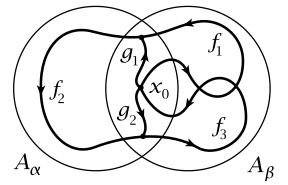
\includegraphics[width=0.4\textwidth]{lemma115.png}
     \label{fig:lemma115-png}
 \end{figure}

 \textbf{Corollary 1.16:} $\mathbb{R}^2$ is not homeomorphic to
 $\mathbb{R}^{n}$ for $n\neq 2$.\\
 \linebreak
 The more general statement that $\mathbb{R}^{m}$ is not homeomorphic to
 $\mathbb{R}^{n}$ if $m\neq n$ can be proved in the same way using either the
 higher homotopy groups or homology groups. In fact, nonempty open sets in
 $\mathbb{R}^{m}$ and $\mathbb{R}^{n}$ can be homeomorphic only if $m = n$, as
 we will see in theorem 2.26 using homology.\\
 \linebreak
 \textbf{Proposition 1.17:} If a space $X$ retracts onto a subspace $A$, then
 the homomorphism $i_*  \colon \pi_1 \left( A, x_0 \right) \to 
 \pi_1 \left( X, x_0 \right) $ induced by the inclusion $i  \colon
 A \to X$ is injective. If $A$ is a deformation retract of $X$, then $i_*$ is
 an isomorphism.\\
 \linebreak
 \textbf{Proof:} If $r  \colon X \to A$ is a retraction, then
 $r i = \mathbbm{1}$, hence $r_* i_* = \mathbbm{1}$, which implies that
 $i_*$ is injective. If $r_t  \colon X\to X$ is a deformation retraction of
 $X$ onto $A$, so $r_0 = \mathbbm{1}, r_t|_{A} = \mathbbm{1}$, and $r_1(X)
 \subset A$, then for any loop $f \colon I \to X$ based at $x_0 \in A$ the
 composition $r_t f$ gives a homotopy of $f$ to a loop in $A$, so $i_*$ is also
 surjective.\\
 \linebreak
 This gives another way of seeing that $S^{1}$ is not a retract of $D^2$ :
 the inclusion-induced map $\pi_1 (S^{1}) \to \pi_1 \left( D^2 \right) $ 
 is a homomorphism $\mathbb{Z} \to 0$ which cannot be injective.\\
 \linebreak
 If $\varphi_t  \colon X \to Y$ is a homotopy that takes a subspace
 $A \subset X$ to a subspace $B \subset Y$ for all $t$, then we speak of
 a homotopy of maps of pairs, $\varphi_t  \colon \left( X,A \right) \to \left(
 Y,B\right) $. In particular, a \textbf{basepoint-preserving homotopy}
 $\varphi_t  \colon \left( X, x_0 \right) \to \left( Y, y_0 \right) $ is the
 case that $\varphi_t (x_0) = y_0$ for all $t$. We have:
\begin{itemize}
    \item If $\varphi_t  \colon \left( X, x_0 \right) \to \left( Y, y_0 \right) $ 
        is a basepoint-preserving homotopy, then
        $\varphi_{0*} = \varphi_{1*}$,
\end{itemize}
since $\varphi_{0*}\left[ f \right]  = \left[ \varphi_0 f \right] = 
\left[ \varphi_1 f \right] = \varphi_{1*} \left[ f \right] $.\\
\linebreak
There is a notion of homotopy equivalence for spaces with basepoints. One says
$\left( X, x_0 \right) \simeq \left( Y, y_0 \right) $ if there are maps
$\varphi  \colon \left( X, x_0 \right)  \to \left( Y, y_0 \right) $ and
$\psi  \colon \left( Y, y_0 \right) \to \left( X, x_0 \right) $ 
with homotopies $\varphi \psi \simeq \mathbbm{1}$ and $\psi \varphi \simeq
\mathbbm{1}$ through maps fixing the basepoints.\\
Then the induced maps on $\pi_1$ satisfy $\varphi_* \psi_* = 
\left( \varphi \psi \right)_* = \mathbbm{1}_* = \mathbbm{1} $ and likewise
$\psi_* \varphi_* = \mathbbm{1}$, so $\varphi_*$ and $\psi_*$ are inverse
isomorphisms $\pi_1 \left( X, x_0 \right) 
\approx \pi_1 \left( Y, y_0 \right) $.\\
\linebreak
This gives another proof that a deformation retraction induces an isomorphism
on
fundamental groups, since if $X$ deformation retracts onto $A$ then
$\left( X, x_0 \right) \simeq \left( A, x_0 \right) $ for any choice of
basepoint $x_0 \in A$.\\
\linebreak
Having to pay so much attention to basepoints when dealing with the fundamental
group is something of a nuisance. For homotopy equivalence one does not have to
be quite so careful:\\
\linebreak
\textbf{Proposition 1.18:} If $\varphi  \colon X\to Y$ is a homotopy
equivalence, then the induced homomorphism $\varphi_*  \colon
\pi_1 \left( X, x_0 \right) \to \pi \left( Y, \varphi(x_0) \right) $ is an
isomorphism for all $x_0 \in X$.\\
\linebreak
\textbf{Lemma 1.19:} If $\varphi_t  \colon X\to Y$ is a homotopy and $h$ is the
path $\varphi_t (x_0)$ formed by the images of a basepoint $x_0 \in X$, then
the three maps in the diagram satisfy $\varphi_{0*} = \beta_h \varphi_{1*}$.
\begin{figure}[H]
    \centering
    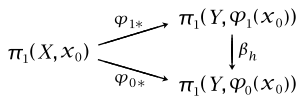
\includegraphics[width=0.4\textwidth]{lemma119.png}
    \label{fig:lemma119-png}
\end{figure}
\textbf{Proof:} Let $h_t$ be the restriction of $h$ to the interval $\left[ 0,t
\right] $,
with a reparametrization so that the domain of $h_t$ is still 
 $\left[ 0,1 \right] $. Explicitly, we can take $h_t (s) = h(ts)$. Then
 if $f$ is a loop in $X$ at the basepoint $x_0$, the product 
 $h_t \cdot \left( \varphi_t f \right) \cdot \overline{h_t}$ gives
 a homotopy of loops at $\varphi_0 (x_0)$ (see figure). Restricting this
 homotopy to $t=0$ and $t=1$, we see that $\varphi_{0*}\left( \left[ f \right]  \right) 
 = \beta_h \left( \varphi_{1*}\left( \left[ f \right]  \right)  \right) $.

\begin{figure}[H]
    \centering
    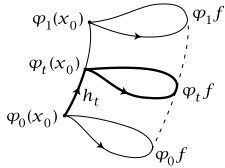
\includegraphics[width=0.3\textwidth]{lemma119-2.png}
    \label{fig:lemma119-2-png}
\end{figure}


\subsection*{Lecture 4 - Van Kampen's Theorem}

Methods to find presentations of $\pi \left( X, x_0 \right) $.
Group presentations: like $\langle r,s  \mid \text{conditions} \rangle$.\\
\linebreak
\textbf{Free products groups:} Given a collection of groups $\left\{ G_{\alpha}
\right\}_{\alpha \in A}$, we can form the free product
$\ast_{\alpha}G_{\alpha}$ as follows: as a set, the free product
$*_{\alpha}G_{\alpha}$ consists of all words $g_1 g_2 \ldots g_m$ of arbitrary
finite length $m\ge 0$, where each letter $g_i$ belonds to a group
$G_{\alpha_i}$ and is not the identity element of $G_{\alpha_{i}}$, and
adjacent letters $g_i$ and $g_{i+1}$ belong to different groups $G_{\alpha}$,
that is, $\alpha_i \neq \alpha_{i+1}$. Words satisfying these conditions are
called \textit{reduced}.
The empty word is allowed, and will be the identity element of 
$*_{\alpha}G_{\alpha}$. The group operation in $*_{\alpha}G_{\alpha}$ is
juxaposition,
$\left( g_1 \ldots g_m \right) \left( h_1 \ldots h_n \right) 
= g_1 \ldots g_m h_1 \ldots h_n$.\\
\linebreak
In particular, we have the free product $\mathbb{Z} * \mathbb{Z}$ as described
on p. 40. The elements of a free group are uniquely representable as reduced
words in powers of generators for various copies of $\mathbb{Z}$, with one
generator for each $\mathbb{Z}$. These generators are called a \textit{basis}
for the free group, and the number of basis elements is the \textit{rank} of
the free group. The abelianization of a free group is a free abelian group with
basis the same set of generators, so since the rank of a free abelian group is
well-defined, independent of the choice of basis, the same is true for the rank
of a free group.\\
\linebreak
A basic property of the free product $*_{\alpha}G_{\alpha}$ is that any
collection of homomorphisms $\varphi_{\alpha}  \colon G_{\alpha} \to H$ extends
uniquely to a homomorphism
$\varphi  \colon *_{\alpha}G_{\alpha} \to H$. Namely, the value of 
$\varphi$ on $g_1 \ldots g_n$ with $g_i \in G_{\alpha_i}$ must be
$\varphi_{\alpha_1} (g_1) \ldots \varphi_{\alpha_n} (g_n)$. For example,
for the free product $G*H$, the inclusions $G \to G \times H$ and 
$H \to G \times H$ induce a surjective homomorphism $G*H \to G \times H$.

\subsubsection*{The Van Kampen Theorem}
Suppose a space $X$ decomposes as the union of a collection of path-connected
open subsets $A_{\alpha}$, each of which contains the basepoint $x_0 \in X$.
Then the homomorphisms $j_{\alpha}  \colon \pi_1 \left( A_{\alpha} \right) 
\to \pi_1 \left( X \right) $ induced by the inclusions
$A_{\alpha} \to X$ extend to a homomorphism $\Phi  \colon 
*_{\alpha} \pi_1 \left( A_{\alpha} \right) \to \pi_1 (X)$. 
The van Kampen theorem will say that $\Phi$ is very often surjective, but we
can expect $\Phi$ to have a nontrivial kernel in general. For if
$i_{\alpha \beta}  \colon \pi_1 \left( A_{\alpha} \cap A_{\beta} \right) 
\to \pi_1 \left( A_{\alpha} \right) $ is the homomorphism induced by the
inclusion
$A_{\alpha} \cap A_{\beta} \to A_{\alpha}$ then
$j_{\alpha} i_{\alpha \beta} = j_{\beta} i_{\beta \alpha}$, both these
compositions being induced by the inclusion $A_{\alpha} \cap A_{\beta} \to X$,
so the kernel of $\Phi$ contains all the elements of the form
$i_{\alpha \beta}(\omega) i_{\beta \alpha} \left( \omega \right)^{-1}$ for
$\omega \in \pi_1 \left( A_{\alpha} \cap A_{\beta} \right) $. Van Kampen's
theorem asserts that under fairly broad hypotheses this gives a full
description of
$\Phi$ :\\
\linebreak

\textbf{Theorem 1.20:} If $X$ is the union of path-connected open sets
$A_{\alpha}$ each containing the basepoint $x_0 \in X$ and if each intersection
$A_{\alpha} \cap A_{\beta}$ is path-connected, then the
homomorphism $\Phi  \colon *_{\alpha}\pi_1 \left( A_{\alpha} \right) 
\to \pi_1 \left( X \right) $ is surjective. If in addition each intersection
$A_{\alpha} \cap A_{\beta} \cap A_{\gamma}$ is path-connected, then the kernel
of $\Phi$ is the normal subgroup $N$ generated by all elements of the form
$i_{\alpha \beta} (\omega) i_{\beta \alpha}\left( \omega \right)^{-1}$ for
$\omega \in \pi_1 \left( A_{\alpha} \cap A_{\beta} \right) $, and
hence $\Phi$ induces an isomorphism $\pi_1 \left( X \right) \approx
*_{\alpha} \pi_1 \left( A_{\alpha} \right) / N$.





\textbf{Fischer-Zastrow}


\newpage

If $Y$ is a spanning tree of $X$, each edge in
$X - Y$ gives a loop going through $x_0$.\\
\linebreak
Can 1A.4 be used to show every subgroup of a free abelian group
is free abelian?\\

\linebreak
Reidemeister Schreier algorithm: find gen. set. for finite-index
subgroups of a free group.\\
\linebreak
Sphere theorem of Papakyriokopoulos. 













\end{document}
